\documentclass[a4 paper,12pt]{article}
\usepackage[inner=2.0cm,outer=2.0cm,top=2.0cm,bottom=2.0cm]{geometry}
\linespread{1.1}
\usepackage{setspace}
\usepackage[rgb]{xcolor}
\usepackage{verbatim}
\usepackage{subcaption}
\usepackage{longtable}
\usepackage{fancyhdr}
\usepackage{fullpage}
\usepackage[colorlinks=true, urlcolor=blue, linkcolor=blue, citecolor=blue]{hyperref}
\usepackage{booktabs}
\usepackage{amsmath,amsfonts,amsthm,amssymb}
\usepackage[shortlabels]{enumitem}
\usepackage{setspace}
\usepackage{extramarks}
\usepackage{soul,color}
\usepackage{graphicx,float,wrapfig}
\usepackage{tikz}
\usepackage{pgfplots}
\usepackage{amsmath}

\newenvironment{breakablealgorithm}
  {% \begin{breakablealgorithm}
   \begin{center}
     \refstepcounter{algorithm}% New algorithm
     \hrule height.8pt depth0pt \kern2pt% \@fs@pre for \@fs@ruled
     \renewcommand{\caption}[2][\relax]{% Make a new \caption
       {\raggedright\textbf{\ALG@name~\thealgorithm} ##2\par}%
       \ifx\relax##1\relax % #1 is \relax
         \addcontentsline{loa}{algorithm}{\protect\numberline{\thealgorithm}##2}%
       \else % #1 is not \relax
         \addcontentsline{loa}{algorithm}{\protect\numberline{\thealgorithm}##1}%
       \fi
       \kern2pt\hrule\kern2pt
     }
  }{% \end{breakablealgorithm}
     \kern2pt\hrule\relax%
   \end{center}
  }
\makeatother
\newtheoremstyle{definitionstyle}
  {3pt} % Space above
  {3pt} % Space below
  {\normalfont} % Body font
  {} % Indent amount
  {\bfseries} % Theorem head font
  {} % Punctuation after theorem head
  { } % Space after theorem head
  {} % Theorem head spec (can be left empty, meaning `normal`)

\theoremstyle{definitionstyle}
\newtheorem{defn}{Definition}
\newtheorem{thm}{Theorem}
\newtheorem{lem}{Lemma}
\newtheorem{statement}{Statement}
% \newtheorem{proof}{Proof}
\usepackage{framed}
\newenvironment{framedminipage}
    {\begin{framed}\begin{minipage}{0.9\textwidth}}
    {\end{minipage}\end{framed}}
\newcommand{\homework}[3]{
	\pagestyle{myheadings}
	\thispagestyle{plain}
	\newpage
	\setcounter{page}{1}
	\noindent
	\begin{center}
		\framebox{
			\vbox{\vspace{2mm}
				\hbox to 6.28in { {\bf Deep Learning \hfill} {\hfill {\rm #2} {\rm #3}} }
				\vspace{4mm}
				\hbox to 6.28in { {\Large \hfill #1  \hfill} }
				\vspace{3mm}}
		}
	\end{center}
	\vspace*{4mm}
}
\newcommand\numberthis{\addtocounter{equation}{1}\tag{\theequation}}

\begin{document}
\homework{CP3 Report}{2024011303}{Liu Hanzuo}
\section*{EBM}
Here we show the result of EBM:
\begin{figure}[H]
    \centering
    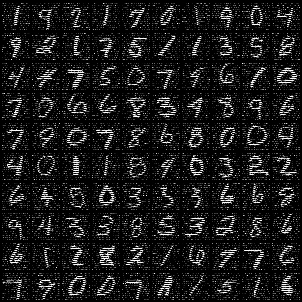
\includegraphics[width=0.8\textwidth]{ebm/data_corrupted.png}
    \caption{corrupted data from EBM}
    \label{corrupted}
\end{figure}
\begin{figure}[H]
    \centering
    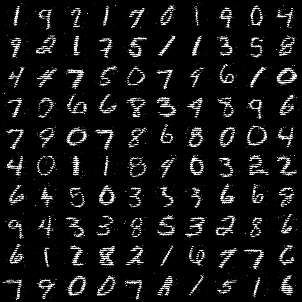
\includegraphics[width=0.8\textwidth]{ebm/data_recovered.png}
    \caption{recovered data from EBM}
    \label{recovered}
\end{figure}
The recovered MSE of the picture is 0.031, while the corrupted MSE is 0.063.
\section*{GAN}
Here we show the result of GAN:
\begin{figure}[H]
    \centering
    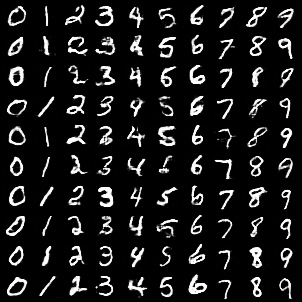
\includegraphics[width=0.8\textwidth]{gan/sample.png}
    \caption{sample from GAN}
    \label{gan}
\end{figure}
\begin{figure}[H]
    \centering
    \begin{tabular}{ccccc}
        
\includegraphics[width=0.18\textwidth]{gan/generated/1/1_020.png} &
        
\includegraphics[width=0.18\textwidth]{gan/generated/2/2_000.png} &
        
\includegraphics[width=0.18\textwidth]{gan/generated/3/3_010.png} &
        
\includegraphics[width=0.18\textwidth]{gan/generated/4/4_020.png} &
        
\includegraphics[width=0.18\textwidth]{gan/generated/5/5_050.png} \\
        
\includegraphics[width=0.18\textwidth]{gan/generated/6/6_010.png} &
        
\includegraphics[width=0.18\textwidth]{gan/generated/7/7_050.png} &
        
\includegraphics[width=0.18\textwidth]{gan/generated/8/8_020.png} &
        
\includegraphics[width=0.18\textwidth]{gan/generated/9/9_017.png} &
    \end{tabular}
    \caption{Generated images from GAN}
    \label{gan_generated}
\end{figure}
The std is shown in the below table:
\begin{table}[H]
    \centering
    \begin{tabular}{|c|c|c|}
        \hline
        Number & Standard Deviation & Requirements\\ \hline
        0 & 0.1719 & 0.17 \\\hline
        1 & 0.0920 & 0.08 \\ \hline
        2 & 0.1811 & 0.17 \\ \hline
        3 & 0.1639 & 0.15 \\ \hline
        4 & 0.1588 & 0.14 \\ \hline
        5 & 0.1733 & 0.16 \\ \hline
        6 & 0.1609 & 0.15 \\ \hline
        7 & 0.1470 & 0.13 \\\hline
        8 & 0.1689 & 0.15 \\\hline
        9 & 0.1407 & 0.13 \\\hline
    \end{tabular}
    \caption{Standard deviation of generated numbers from GAN}
    \label{std_table}
\end{table}
The FID score for the 10 classes is as follows:
\begin{table}[H]
    \centering
    \begin{tabular}{|c|c|}
        \hline
        Class & FID Score \\ \hline
        0 & 5.599 \\ \hline
        1 & 8.525 \\ \hline
        2 & 10.571 \\ \hline
        3 & 5.246 \\ \hline
        4 & 10.545 \\ \hline
        5 & 15.946\\ \hline
        6 & 4.126 \\ \hline
        7 & 9.902\\ \hline
        8 & 7.992 \\ \hline
        9 & 8.480
         \\ \hline
    \end{tabular}
    \caption{FID scores for 10 classes}
    \label{fid_table}
\end{table}
\end{document} 
